\documentclass[11pt,a4paper]{article}

%==============================================================================
% PACKAGES
%==============================================================================
\usepackage[utf8]{inputenc}
\usepackage[T1]{fontenc}
\usepackage{amsmath,amssymb,amsfonts}
\usepackage{graphicx}
\usepackage{booktabs}
\usepackage{longtable}
\usepackage{array}
\usepackage{hyperref}
\usepackage{xcolor}
\usepackage{geometry}
\usepackage{fancyhdr}
\usepackage{listings}
\usepackage{tcolorbox}
\usepackage{enumitem}
\usepackage{tikz}
\usepackage{pdflscape}
\usepackage{multicol}
\usepackage{titlesec}
\usetikzlibrary{shapes,arrows,positioning,calc}

%==============================================================================
% PAGE SETUP
%==============================================================================
\geometry{margin=1in, top=1.2in, bottom=1in}
\pagestyle{fancy}
\fancyhf{}
\fancyhead[L]{\leftmark}
\fancyhead[R]{Optimized Checkout System}
\fancyfoot[C]{Page \thepage}
\fancyfoot[R]{\footnotesize Confidential}

\setlength{\headheight}{14pt}

%==============================================================================
% COLORS
%==============================================================================
\definecolor{primaryblue}{RGB}{41,128,185}
\definecolor{secondaryblue}{RGB}{52,152,219}
\definecolor{successgreen}{RGB}{39,174,96}
\definecolor{warningorange}{RGB}{230,126,34}
\definecolor{dangerred}{RGB}{192,57,43}
\definecolor{codegray}{RGB}{245,245,245}
\definecolor{darkgray}{RGB}{80,80,80}
\definecolor{lightgray}{RGB}{220,220,220}

%==============================================================================
% HYPERREF SETUP
%==============================================================================
\hypersetup{
    colorlinks=true,
    linkcolor=primaryblue,
    urlcolor=secondaryblue,
    citecolor=successgreen
}

%==============================================================================
% CODE LISTING STYLE
%==============================================================================
\lstset{
    backgroundcolor=\color{codegray},
    basicstyle=\ttfamily\small,
    breaklines=true,
    frame=single,
    numbers=left,
    numberstyle=\tiny\color{gray},
    keywordstyle=\color{primaryblue}\bfseries,
    commentstyle=\color{successgreen},
    stringstyle=\color{warningorange},
    showstringspaces=false,
    tabsize=4
}

%==============================================================================
% CUSTOM TCOLORBOXES
%==============================================================================
\tcbuselibrary{skins,breakable}

\newtcolorbox{executivebox}{
    colback=primaryblue!5,
    colframe=primaryblue,
    title=Executive Summary,
    fonttitle=\bfseries\large,
    breakable
}

\newtcolorbox{keyinsight}{
    colback=primaryblue!10,
    colframe=primaryblue,
    title=Key Insight,
    fonttitle=\bfseries,
    breakable
}

\newtcolorbox{requirementbox}[1]{
    colback=secondaryblue!5,
    colframe=secondaryblue,
    title=#1,
    fonttitle=\bfseries,
    breakable
}

\newtcolorbox{metricbox}{
    colback=successgreen!10,
    colframe=successgreen,
    title=Success Metrics,
    fonttitle=\bfseries,
    breakable
}

\newtcolorbox{warningbox}{
    colback=warningorange!10,
    colframe=warningorange,
    title=Warning,
    fonttitle=\bfseries,
    breakable
}

\newtcolorbox{decisionbox}{
    colback=successgreen!10,
    colframe=successgreen,
    title=Decision Rule,
    fonttitle=\bfseries,
    breakable
}

\newtcolorbox{riskbox}{
    colback=dangerred!10,
    colframe=dangerred,
    title=Risk Alert,
    fonttitle=\bfseries,
    breakable
}

\newtcolorbox{phasebox}[1]{
    colback=lightgray!30,
    colframe=darkgray,
    title=#1,
    fonttitle=\bfseries,
    breakable
}

%==============================================================================
% TITLE FORMATTING
%==============================================================================
\titleformat{\section}
    {\normalfont\Large\bfseries\color{primaryblue}}
    {\thesection}{1em}{}
\titleformat{\subsection}
    {\normalfont\large\bfseries\color{darkgray}}
    {\thesubsection}{1em}{}
\titleformat{\subsubsection}
    {\normalfont\normalsize\bfseries}
    {\thesubsubsection}{1em}{}

%==============================================================================
% DOCUMENT INFO
%==============================================================================
\title{
    \vspace{-2cm}
    \includegraphics[width=0.15\textwidth]{example-image}\\[1em]
    {\Huge\bfseries\color{primaryblue} Optimized Checkout}\\[0.5em]
    {\Large System Design Document}\\[0.5em]
    {\large Product Requirements, A/B Testing Methodology,}\\
    {\large and Implementation Roadmap}\\[2em]
    \rule{\textwidth}{1pt}
}

\author{
    \textbf{Contributors:}\\[0.5em]
    Product Manager Agent $\cdot$ Statistics Agent $\cdot$ Psychology Agent\\[1em]
    \textit{Multi-Agent Research System}
}

\date{
    \vspace{1em}
    January 2026\\
    Version 1.0\\[1em]
    \textcolor{dangerred}{\textbf{CONFIDENTIAL}}
}

%==============================================================================
% BEGIN DOCUMENT
%==============================================================================
\begin{document}

% Title page
\maketitle
\thispagestyle{empty}
\newpage

% Document control
\section*{Document Control}
\begin{table}[h]
\centering
\begin{tabular}{@{}ll@{}}
\toprule
\textbf{Item} & \textbf{Details} \\
\midrule
Document Title & Optimized Checkout System Design Document \\
Version & 1.0 \\
Status & Draft for Review \\
Classification & Confidential \\
Owner & Product Management \\
Last Updated & January 1, 2026 \\
\bottomrule
\end{tabular}
\end{table}

\subsection*{Revision History}
\begin{table}[h]
\centering
\begin{tabular}{@{}lllp{6cm}@{}}
\toprule
\textbf{Version} & \textbf{Date} & \textbf{Author} & \textbf{Changes} \\
\midrule
0.1 & 2026-01-01 & PM Agent & Initial PRD draft \\
0.2 & 2026-01-01 & Stats Agent & A/B testing methodology \\
0.3 & 2026-01-01 & Psych Agent & Behavioral considerations \\
1.0 & 2026-01-01 & PM Agent & Unified system document \\
\bottomrule
\end{tabular}
\end{table}

\subsection*{Approval}
\begin{table}[h]
\centering
\begin{tabular}{@{}llll@{}}
\toprule
\textbf{Role} & \textbf{Name} & \textbf{Signature} & \textbf{Date} \\
\midrule
Product Lead & & & \\
Engineering Lead & & & \\
Data Science Lead & & & \\
Design Lead & & & \\
\bottomrule
\end{tabular}
\end{table}

\newpage

% Table of contents
\tableofcontents
\newpage

%##############################################################################
% PART I: EXECUTIVE OVERVIEW
%##############################################################################
\part{Executive Overview}

\section{Executive Summary}

\begin{executivebox}
The \textbf{Optimized Checkout} feature represents a strategic initiative to reduce cart abandonment and increase e-commerce conversion rates through evidence-based design principles. This system document provides a comprehensive framework covering product requirements, experimentation methodology, and implementation roadmap.
\end{executivebox}

\subsection{Strategic Context}

Cart abandonment remains one of the most significant challenges in e-commerce, with industry-wide rates averaging 70\%. Our analysis indicates that checkout friction---driven by cognitive overload, decision fatigue, and poor UX---is a primary contributor.

\subsection{Research Foundation}

This initiative is grounded in peer-reviewed research from psychiatry and cognitive psychology:

\begin{table}[h]
\centering
\begin{tabular}{@{}lp{8cm}@{}}
\toprule
\textbf{Research Domain} & \textbf{Application} \\
\midrule
Decision-making \& Impulse Control \newline (Bechara, 2005) & Humans prefer immediate gratification; reducing friction enables faster purchase decisions \\
\addlinespace
Cognitive Load Theory \newline (Sweller, 1988) & Working memory overload decreases satisfaction; simplification improves conversion \\
\addlinespace
Attention \& Visual Processing & Colors, movement, and relevance direct user focus to key actions \\
\addlinespace
Reward Systems \newline (Berridge, 2007) & Anticipation of reward drives engagement; applies to checkout completion \\
\bottomrule
\end{tabular}
\caption{Research foundations informing feature design}
\end{table}

\subsection{Target Outcomes}

\begin{metricbox}
\begin{tabular}{@{}lllc@{}}
\toprule
\textbf{Metric} & \textbf{Current} & \textbf{Target} & \textbf{Impact} \\
\midrule
Cart abandonment rate & 70\% & 50\% & -20 pts \\
Checkout completion time & 4.5 min & 1.5 min & -67\% \\
Conversion rate & 2.5\% & 2.75\% & +10\% \\
Customer satisfaction (CSAT) & 6.5/10 & 8.0/10 & +23\% \\
\bottomrule
\end{tabular}
\end{metricbox}

\subsection{Approach}

Our approach integrates three disciplines:

\begin{enumerate}
    \item \textbf{Product Management:} Define requirements based on user needs and business objectives
    \item \textbf{Data Science:} Design rigorous A/B testing with early-stopping strategies
    \item \textbf{Psychology:} Account for cognitive biases and novelty effects in experimentation
\end{enumerate}

\subsection{Document Structure}

\begin{table}[h]
\centering
\begin{tabular}{@{}clp{7cm}@{}}
\toprule
\textbf{Part} & \textbf{Title} & \textbf{Contents} \\
\midrule
I & Executive Overview & Summary, context, outcomes \\
II & Product Requirements & User stories, functional specs, UX guidelines \\
III & A/B Testing Methodology & Experiment design, early stopping, metrics \\
IV & Implementation & Roadmap, RACI, decision framework \\
V & Appendices & Code, glossary, references \\
\bottomrule
\end{tabular}
\caption{Document structure}
\end{table}

\newpage

%##############################################################################
% PART II: PRODUCT REQUIREMENTS
%##############################################################################
\part{Product Requirements Document}

\section{Problem Statement}

\subsection{Current State Analysis}

Users encounter a lengthy checkout process with irrelevant information and multiple decision points, leading to cognitive overload and purchase abandonment.

\begin{table}[h]
\centering
\begin{tabular}{@{}lr@{}}
\toprule
\textbf{Metric} & \textbf{Current State} \\
\midrule
Average checkout flow & 5+ pages \\
Cart abandonment rate & $\sim$70\% \\
Form fields requiring manual entry & 15+ \\
Decision points causing friction & 8+ \\
Average completion time & 4.5 minutes \\
\bottomrule
\end{tabular}
\caption{Current checkout performance metrics}
\end{table}

\subsection{User Pain Points}

\begin{table}[h]
\centering
\begin{tabular}{@{}lp{9cm}@{}}
\toprule
\textbf{Persona} & \textbf{Pain Points} \\
\midrule
Casual Shopper & Distracted by irrelevant options, complex UI, loses purchase momentum, experiences choice paralysis \\
Streamlined Shopper & Frustrated by multiple steps, time-consuming checkout, repetitive data entry, unnecessary validation \\
Anxious Buyer & Worried about security, unclear about total cost, unsure about return policy, needs reassurance \\
\bottomrule
\end{tabular}
\caption{Pain points by user persona}
\end{table}

\section{User Stories \& Use Cases}

\subsection{User Stories}

\begin{requirementbox}{Priority 0 (Must Have)}
\begin{description}[style=nextline,leftmargin=1cm]
    \item[US-001] As a \textbf{Casual Shopper}, I want to easily modify my cart items so I can impulsively add or remove items without leaving checkout.

    \item[US-002] As a \textbf{Streamlined Shopper}, I need a one-page checkout so that I can quickly complete my purchase.

    \item[US-003] As a \textbf{returning customer}, I want my payment and shipping info pre-filled so I don't waste time re-entering data.
\end{description}
\end{requirementbox}

\begin{requirementbox}{Priority 1 (Should Have)}
\begin{description}[style=nextline,leftmargin=1cm]
    \item[US-004] As a \textbf{mobile user}, I want large tap targets and minimal typing so I can checkout easily on my phone.

    \item[US-005] As an \textbf{anxious buyer}, I want clear progress indicators so I know exactly where I am in the process.

    \item[US-006] As a \textbf{guest user}, I want to checkout without creating an account so I can complete my purchase quickly.
\end{description}
\end{requirementbox}

\subsection{Use Cases}

\subsubsection{UC-001: Express Checkout (Returning Customer)}

\textbf{Preconditions:} User is logged in with saved payment and shipping information.

\begin{enumerate}
    \item User adds item to cart
    \item User clicks ``Buy Now'' button
    \item System displays one-page checkout with pre-filled data
    \item User reviews order summary
    \item User confirms payment method (saved card with last 4 digits visible)
    \item User clicks ``Place Order''
    \item System processes payment and displays confirmation
    \item Order confirmed in $<$30 seconds total
\end{enumerate}

\textbf{Postconditions:} Order created, confirmation email sent, inventory updated.

\subsubsection{UC-002: Guest Checkout}

\textbf{Preconditions:} User has items in cart, not logged in.

\begin{enumerate}
    \item User clicks ``Proceed to Checkout''
    \item System displays checkout with prominent ``Guest Checkout'' option
    \item User selects guest checkout
    \item User enters email, shipping address, payment info (minimal fields)
    \item System validates in real-time (inline errors)
    \item User reviews order and clicks ``Place Order''
    \item System offers to save info for future (optional account creation)
    \item Order confirmed
\end{enumerate}

\textbf{Postconditions:} Order created, guest account optionally converted.

\section{Functional Requirements}

\subsection{One-Page Checkout (FR-1xx)}

\begin{table}[h]
\centering
\begin{tabular}{@{}clc@{}}
\toprule
\textbf{ID} & \textbf{Requirement} & \textbf{Priority} \\
\midrule
FR-101 & Consolidate entire checkout into single scrollable page & P0 \\
FR-102 & Implement accordion sections for Shipping, Payment, Review & P0 \\
FR-103 & Display sticky order summary visible at all scroll positions & P0 \\
FR-104 & Provide real-time inline validation (not on submit) & P0 \\
FR-105 & Auto-expand next section on completion of current & P1 \\
FR-106 & Allow manual section expansion/collapse & P1 \\
\bottomrule
\end{tabular}
\caption{One-page checkout requirements}
\end{table}

\subsection{Auto-Fill \& Smart Defaults (FR-2xx)}

\begin{table}[h]
\centering
\begin{tabular}{@{}clc@{}}
\toprule
\textbf{ID} & \textbf{Requirement} & \textbf{Priority} \\
\midrule
FR-201 & Auto-fill from saved user profile for logged-in users & P0 \\
FR-202 & Support browser autofill via proper autocomplete attributes & P0 \\
FR-203 & Integrate Google Places API for address autocomplete & P1 \\
FR-204 & Pre-select default shipping method based on user history & P1 \\
FR-205 & Remember last-used payment method & P1 \\
\bottomrule
\end{tabular}
\caption{Auto-fill requirements}
\end{table}

\subsection{Dynamic Cart Modifications (FR-3xx)}

\begin{table}[h]
\centering
\begin{tabular}{@{}clc@{}}
\toprule
\textbf{ID} & \textbf{Requirement} & \textbf{Priority} \\
\midrule
FR-301 & Enable inline quantity adjustment without page reload & P0 \\
FR-302 & Provide one-click item removal with 5-second undo option & P0 \\
FR-303 & Update order total in real-time on cart changes & P0 \\
FR-304 & Implement ``Save for later'' functionality & P2 \\
\bottomrule
\end{tabular}
\caption{Cart modification requirements}
\end{table}

\subsection{Visual Feedback \& Attention (FR-4xx)}

\begin{table}[h]
\centering
\begin{tabular}{@{}clc@{}}
\toprule
\textbf{ID} & \textbf{Requirement} & \textbf{Priority} \\
\midrule
FR-401 & Style primary CTA button with high-contrast brand color & P0 \\
FR-402 & Display trust badges (SSL, payment logos) near payment section & P0 \\
FR-403 & Show progress indicator for multi-section flow & P1 \\
FR-404 & Add micro-animations for state changes (success, error) & P2 \\
FR-405 & Highlight active form field with visual border & P1 \\
\bottomrule
\end{tabular}
\caption{Visual feedback requirements}
\end{table}

\subsection{Express Checkout Options (FR-5xx)}

\begin{table}[h]
\centering
\begin{tabular}{@{}clc@{}}
\toprule
\textbf{ID} & \textbf{Requirement} & \textbf{Priority} \\
\midrule
FR-501 & Add ``Buy Now'' button on product detail pages & P0 \\
FR-502 & Integrate Apple Pay for iOS/Safari users & P1 \\
FR-503 & Integrate Google Pay for Android/Chrome users & P1 \\
FR-504 & Support PayPal Express Checkout & P1 \\
FR-505 & Enable Shop Pay for Shopify ecosystem & P2 \\
\bottomrule
\end{tabular}
\caption{Express checkout requirements}
\end{table}

\section{Non-Functional Requirements}

\subsection{Performance (NFR-1xx)}

\begin{table}[h]
\centering
\begin{tabular}{@{}cll@{}}
\toprule
\textbf{ID} & \textbf{Requirement} & \textbf{Target} \\
\midrule
NFR-101 & Largest Contentful Paint (LCP) & $< 2.0$ seconds \\
NFR-102 & Time to Interactive (TTI) & $< 2.5$ seconds \\
NFR-103 & First Input Delay (FID) & $< 100$ ms \\
NFR-104 & Cumulative Layout Shift (CLS) & $< 0.1$ \\
NFR-105 & API response time (p95) & $< 200$ ms \\
NFR-106 & Payment processing time & $< 3$ seconds \\
\bottomrule
\end{tabular}
\caption{Performance requirements}
\end{table}

\subsection{Security (NFR-2xx)}

\begin{table}[h]
\centering
\begin{tabular}{@{}cll@{}}
\toprule
\textbf{ID} & \textbf{Requirement} & \textbf{Standard} \\
\midrule
NFR-201 & Payment data handling & PCI-DSS Level 1 \\
NFR-202 & Data transmission encryption & TLS 1.3 minimum \\
NFR-203 & Session management & Secure, HttpOnly, SameSite cookies \\
NFR-204 & Fraud detection & 3D Secure 2.0 integration \\
NFR-205 & Input sanitization & OWASP guidelines \\
\bottomrule
\end{tabular}
\caption{Security requirements}
\end{table}

\subsection{Accessibility (NFR-3xx)}

\begin{table}[h]
\centering
\begin{tabular}{@{}cll@{}}
\toprule
\textbf{ID} & \textbf{Requirement} & \textbf{Standard} \\
\midrule
NFR-301 & WCAG compliance level & AA \\
NFR-302 & Keyboard navigation & Full support, visible focus \\
NFR-303 & Screen reader compatibility & ARIA labels on all elements \\
NFR-304 & Color contrast ratio & Minimum 4.5:1 (text), 3:1 (UI) \\
NFR-305 & Touch target size & Minimum 44x44 pixels \\
\bottomrule
\end{tabular}
\caption{Accessibility requirements}
\end{table}

\section{UX/UI Guidelines}

\subsection{Cognitive Load Reduction Principles}

Based on Sweller's Cognitive Load Theory (1988):

\begin{keyinsight}
\textbf{Core Principle:} Minimize extraneous cognitive load to free working memory for the primary task---completing the purchase.
\end{keyinsight}

\begin{enumerate}
    \item \textbf{Minimize Visual Clutter}
    \begin{itemize}
        \item Display maximum 3-4 form fields visible at once
        \item Use progressive disclosure via accordion sections
        \item Hide optional fields by default (expandable on request)
        \item Remove decorative elements that don't aid completion
    \end{itemize}

    \item \textbf{Leverage Color for Attention Guidance}
    \begin{itemize}
        \item Primary CTA: High-contrast brand color (e.g., \textcolor{successgreen}{\#27AE60})
        \item Error states: Red (\textcolor{dangerred}{\#C0392B}) with descriptive icon
        \item Success states: Green (\textcolor{successgreen}{\#27AE60}) with checkmark
        \item Neutral/secondary elements: Muted grays
    \end{itemize}

    \item \textbf{Establish Clear Typography Hierarchy}
    \begin{itemize}
        \item Section headers: 18px bold
        \item Form labels: 14px medium
        \item Helper text: 12px regular, muted color
        \item CTA buttons: 16px bold
    \end{itemize}
\end{enumerate}

\subsection{Wireframe Layout}

\begin{lstlisting}[caption=Checkout page wireframe structure]
+-----------------------------------------------------------+
|  [Logo]                              [Cart: 2 items]      |
+-----------------------------------------------------------+
|                                                           |
|  +---------------------+   +---------------------------+  |
|  | CHECKOUT            |   | ORDER SUMMARY  [sticky]   |  |
|  |                     |   |                           |  |
|  | v Shipping Address  |   | Item 1            $49.00  |  |
|  |   [Name         ]   |   | Item 2            $36.00  |  |
|  |   [Address      ]   |   | ------------------------- |  |
|  |   [City, ST ZIP ]   |   | Subtotal          $85.00  |  |
|  |                     |   | Shipping           $5.00  |  |
|  | > Payment Method    |   | Tax                $7.65  |  |
|  |                     |   | ========================= |  |
|  | > Review Order      |   | TOTAL             $97.65  |  |
|  |                     |   |                           |  |
|  | +------------------+|   | [Visa] [MC] [Amex] [Lock] |  |
|  | |   PLACE ORDER   ||   +---------------------------+  |
|  | +------------------+|                                  |
|  +---------------------+                                  |
+-----------------------------------------------------------+
\end{lstlisting}

\newpage

%##############################################################################
% PART III: A/B TESTING METHODOLOGY
%##############################################################################
\part{A/B Testing Methodology}

\section{Experiment Design}

\subsection{Hypothesis}

\begin{align}
    H_0&: \pi_{\text{treatment}} = \pi_{\text{control}} \quad \text{(no effect on conversion)} \\
    H_1&: \pi_{\text{treatment}} > \pi_{\text{control}} \quad \text{(treatment improves conversion)}
\end{align}

Where $\pi$ represents the checkout conversion rate (orders / checkout sessions).

\subsection{Sample Size Calculation}

For a two-proportion z-test:

\begin{table}[h]
\centering
\begin{tabular}{@{}ll@{}}
\toprule
\textbf{Parameter} & \textbf{Value} \\
\midrule
Baseline conversion rate ($p_1$) & 2.5\% \\
Minimum Detectable Effect (MDE) & 10\% relative lift \\
Target conversion rate ($p_2$) & 2.75\% \\
Significance level ($\alpha$) & 0.05 (two-tailed) \\
Statistical power ($1-\beta$) & 0.80 \\
\bottomrule
\end{tabular}
\caption{Sample size calculation parameters}
\end{table}

The required sample size per arm:

\begin{equation}
n = \frac{2 \cdot (Z_{\alpha/2} + Z_{\beta})^2 \cdot \bar{p}(1-\bar{p})}{(p_2 - p_1)^2}
\end{equation}

Where $Z_{\alpha/2} = 1.96$, $Z_{\beta} = 0.84$, and $\bar{p} = 0.02625$:

\begin{equation}
n \approx \frac{2 \cdot (1.96 + 0.84)^2 \cdot 0.02625 \cdot 0.97375}{(0.0025)^2} \approx 25{,}000 \text{ per arm}
\end{equation}

\begin{decisionbox}
\textbf{Required Sample Size:} $\sim$50,000 unique checkout sessions (25,000 per arm)
\end{decisionbox}

\subsection{Randomization Strategy}

\begin{itemize}
    \item \textbf{Randomization unit:} User ID (cookie-based for guests, account ID for logged-in)
    \item \textbf{Stratification factors:} Device type, customer status (new/returning), region
    \item \textbf{Assignment:} Sticky---users remain in same variant throughout experiment
\end{itemize}

\section{Metrics Framework}

\subsection{Primary Metric}

\begin{table}[h]
\centering
\begin{tabular}{@{}lll@{}}
\toprule
\textbf{Metric} & \textbf{Definition} & \textbf{Success Threshold} \\
\midrule
Checkout Conversion Rate & Orders / Checkout Sessions & $\geq$10\% relative lift, $p < 0.05$ \\
\bottomrule
\end{tabular}
\caption{Primary success metric}
\end{table}

\subsection{Secondary Metrics}

\begin{table}[h]
\centering
\begin{tabular}{@{}lll@{}}
\toprule
\textbf{Metric} & \textbf{Definition} & \textbf{Expected Direction} \\
\midrule
Cart abandonment rate & Abandoned / Started checkouts & Decrease \\
Checkout completion time & Time from cart to order confirmation & Decrease \\
Average order value (AOV) & Revenue / Orders & Neutral or increase \\
Customer satisfaction (CSAT) & Post-checkout survey score (1-10) & Increase \\
\bottomrule
\end{tabular}
\caption{Secondary metrics}
\end{table}

\subsection{Guardrail Metrics}

\begin{riskbox}
If \textbf{any} guardrail metric breaches its threshold, pause or stop the experiment immediately.
\end{riskbox}

\begin{table}[h]
\centering
\begin{tabular}{@{}lll@{}}
\toprule
\textbf{Metric} & \textbf{Threshold} & \textbf{Action} \\
\midrule
Page load time (p95) & $> 3$ seconds & Pause \\
JavaScript error rate & $> 1\%$ & Pause \\
Payment failure rate & $> 2\%$ & \textbf{Stop} \\
Customer support tickets & $> 20\%$ increase & Investigate \\
Revenue per visitor & $> 5\%$ decrease & \textbf{Stop} \\
\bottomrule
\end{tabular}
\caption{Guardrail metrics}
\end{table}

\section{Early Stopping Strategy}

\subsection{The Peeking Problem}

\begin{warningbox}
Continuously monitoring A/B test results inflates false positive rates.\\[0.5em]
\textbf{Example:} Checking daily for 30 days at $\alpha = 0.05$\\
\textbf{Actual Type I error:} $\sim$15--20\% (not 5\%)
\end{warningbox}

\subsection{Group Sequential Design (O'Brien-Fleming)}

We employ the \textbf{O'Brien-Fleming spending function}, which is conservative early and permissive late:

\begin{equation}
\alpha^*(t) = 2 \cdot \left[1 - \Phi\left(\frac{Z_{\alpha/2}}{\sqrt{t}}\right)\right]
\end{equation}

\begin{table}[h]
\centering
\begin{tabular}{@{}ccccc@{}}
\toprule
\textbf{Analysis} & \textbf{Info Fraction} & \textbf{Cumulative $\alpha$} & \textbf{Z-boundary} & \textbf{p-boundary} \\
\midrule
1st (25\%) & 0.25 & 0.0001 & 4.05 & 0.00005 \\
2nd (50\%) & 0.50 & 0.0052 & 2.80 & 0.0051 \\
3rd (75\%) & 0.75 & 0.0184 & 2.28 & 0.0226 \\
Final (100\%) & 1.00 & 0.0500 & 2.02 & 0.0431 \\
\bottomrule
\end{tabular}
\caption{O'Brien-Fleming efficacy boundaries}
\end{table}

\subsection{Futility Stopping}

Stop for futility when conditional power $< 10\%$:

\begin{table}[h]
\centering
\begin{tabular}{@{}cc@{}}
\toprule
\textbf{Analysis} & \textbf{Z for Futility} \\
\midrule
1st (25\%) & $< -0.5$ \\
2nd (50\%) & $< 0.0$ \\
3rd (75\%) & $< 0.5$ \\
\bottomrule
\end{tabular}
\caption{Futility boundaries}
\end{table}

\subsection{Stopping Decision Flowchart}

\begin{figure}[h]
\centering
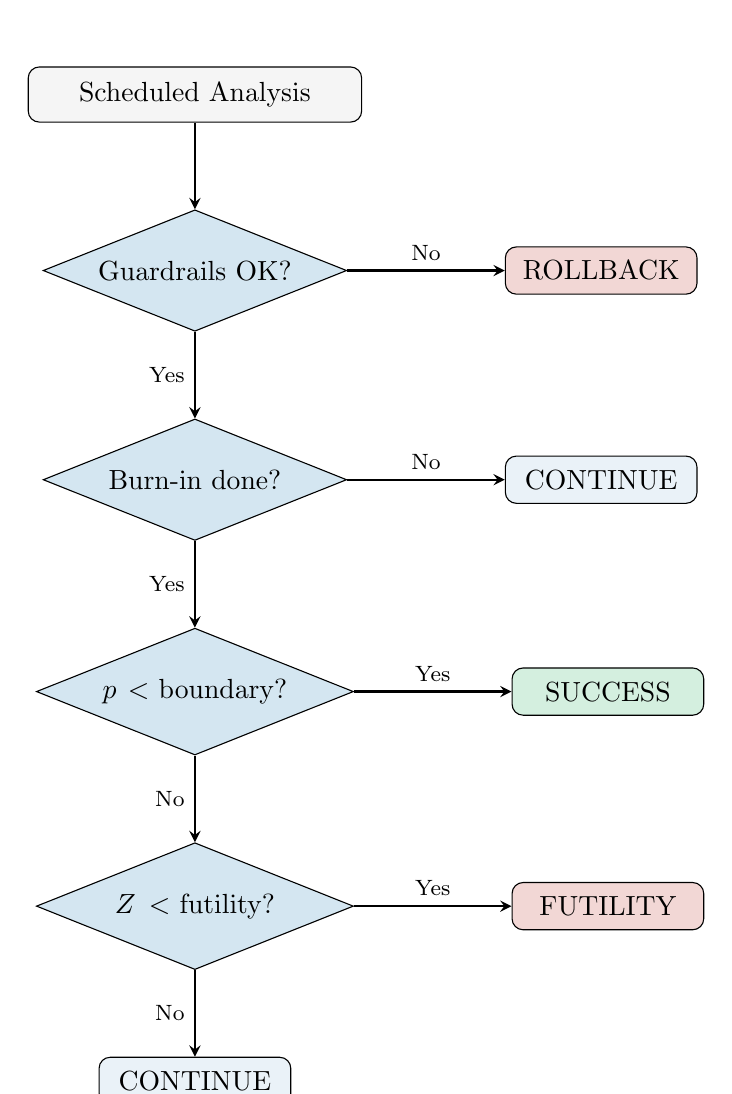
\begin{tikzpicture}[
    node distance=1.1cm,
    decision/.style={diamond, draw, fill=primaryblue!20, text width=3cm, text centered, inner sep=1pt, aspect=2.5},
    block/.style={rectangle, draw, fill=codegray, text width=4cm, text centered, rounded corners, minimum height=0.7cm},
    stop/.style={rectangle, draw, fill=dangerred!20, text width=2.2cm, text centered, rounded corners, minimum height=0.6cm},
    success/.style={rectangle, draw, fill=successgreen!20, text width=2.2cm, text centered, rounded corners, minimum height=0.6cm},
    continue/.style={rectangle, draw, fill=primaryblue!10, text width=2.2cm, text centered, rounded corners, minimum height=0.6cm},
    arrow/.style={thick,->,>=stealth}
]

\node[block] (start) {Scheduled Analysis};
\node[decision, below=of start] (guardrail) {Guardrails OK?};
\node[stop, right=2cm of guardrail] (stop1) {ROLLBACK};
\node[decision, below=of guardrail] (burnin) {Burn-in done?};
\node[continue, right=2cm of burnin] (cont1) {CONTINUE};
\node[decision, below=of burnin] (efficacy) {$p < $ boundary?};
\node[success, right=2cm of efficacy] (stop2) {SUCCESS};
\node[decision, below=of efficacy] (futility) {$Z < $ futility?};
\node[stop, right=2cm of futility] (stop3) {FUTILITY};
\node[continue, below=of futility] (cont2) {CONTINUE};

\draw[arrow] (start) -- (guardrail);
\draw[arrow] (guardrail) -- node[above] {\footnotesize No} (stop1);
\draw[arrow] (guardrail) -- node[left] {\footnotesize Yes} (burnin);
\draw[arrow] (burnin) -- node[above] {\footnotesize No} (cont1);
\draw[arrow] (burnin) -- node[left] {\footnotesize Yes} (efficacy);
\draw[arrow] (efficacy) -- node[above] {\footnotesize Yes} (stop2);
\draw[arrow] (efficacy) -- node[left] {\footnotesize No} (futility);
\draw[arrow] (futility) -- node[above] {\footnotesize Yes} (stop3);
\draw[arrow] (futility) -- node[left] {\footnotesize No} (cont2);

\end{tikzpicture}
\caption{Early stopping decision flowchart}
\end{figure}

\section{Psychological Considerations}

\subsection{Novelty \& Habituation Effects}

\begin{table}[h]
\centering
\begin{tabular}{@{}lll@{}}
\toprule
\textbf{Phase} & \textbf{Duration} & \textbf{Expected Behavior} \\
\midrule
Novelty spike & Days 1--3 & Inflated engagement due to curiosity \\
Learning curve & Days 4--10 & Increased errors as users adapt \\
Habituation & Days 11--14 & Behavior stabilizes toward true effect \\
Steady state & Day 15+ & Reliable measurement period \\
\bottomrule
\end{tabular}
\caption{Novelty effect timeline}
\end{table}

\begin{keyinsight}
\textbf{Recommendation:} Enforce minimum 2-week burn-in before any stopping decisions. Exclude first 3 days from primary analysis. Compare Week 1 vs Week 2 to detect novelty decay.
\end{keyinsight}

\subsection{Cognitive Biases to Monitor}

\begin{table}[h]
\centering
\begin{tabular}{@{}lll@{}}
\toprule
\textbf{Bias} & \textbf{Definition} & \textbf{Measurement} \\
\midrule
Anchoring & Over-reliance on first price seen & Price comparison behavior \\
Loss aversion & Fear of losing deal/item & ``Item removed'' event rate \\
Choice overload & Too many options $\rightarrow$ paralysis & Time-on-page, exit rate \\
Status quo bias & Preference for familiar checkout & Segment by user tenure \\
\bottomrule
\end{tabular}
\caption{Relevant cognitive biases}
\end{table}

\subsection{User Segmentation for Analysis}

\begin{table}[h]
\centering
\begin{tabular}{@{}lll@{}}
\toprule
\textbf{Segment} & \textbf{Behavioral Signals} & \textbf{Expected Response} \\
\midrule
Impulsive shoppers & Fast checkout, few page views & Strong positive \\
Deliberate shoppers & Long sessions, comparisons & Moderate positive \\
Anxious shoppers & High abandonment history & Strong positive (if trust improved) \\
Deal hunters & High coupon usage & Neutral (price $>$ UX) \\
\bottomrule
\end{tabular}
\caption{Psychological segments}
\end{table}

\newpage

%##############################################################################
% PART IV: IMPLEMENTATION
%##############################################################################
\part{Implementation Roadmap}

\section{Phase Overview}

\begin{figure}[h]
\centering
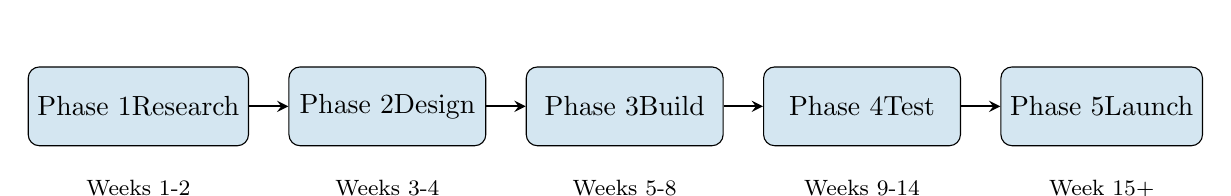
\begin{tikzpicture}[
    phase/.style={rectangle, draw, fill=primaryblue!20, minimum width=2.5cm, minimum height=1cm, text centered, rounded corners},
    arrow/.style={thick,->,>=stealth}
]
\node[phase] (p1) {Phase 1\\Research};
\node[phase, right=0.5cm of p1] (p2) {Phase 2\\Design};
\node[phase, right=0.5cm of p2] (p3) {Phase 3\\Build};
\node[phase, right=0.5cm of p3] (p4) {Phase 4\\Test};
\node[phase, right=0.5cm of p4] (p5) {Phase 5\\Launch};

\draw[arrow] (p1) -- (p2);
\draw[arrow] (p2) -- (p3);
\draw[arrow] (p3) -- (p4);
\draw[arrow] (p4) -- (p5);

\node[below=0.3cm of p1] {\footnotesize Weeks 1-2};
\node[below=0.3cm of p2] {\footnotesize Weeks 3-4};
\node[below=0.3cm of p3] {\footnotesize Weeks 5-8};
\node[below=0.3cm of p4] {\footnotesize Weeks 9-14};
\node[below=0.3cm of p5] {\footnotesize Week 15+};

\end{tikzpicture}
\caption{Implementation phases}
\end{figure}

\section{Detailed Phase Breakdown}

\begin{phasebox}{Phase 1: Research \& Requirements (Weeks 1-2)}
\textbf{Objectives:}
\begin{itemize}
    \item Finalize PRD with stakeholder sign-off
    \item Complete competitive analysis
    \item Define success metrics and guardrails
\end{itemize}

\textbf{Deliverables:}
\begin{itemize}
    \item Approved PRD document
    \item User research synthesis
    \item A/B test plan
\end{itemize}

\textbf{Exit Criteria:} PRD approved by Product Lead, Engineering Lead, Design Lead
\end{phasebox}

\begin{phasebox}{Phase 2: Design \& Prototype (Weeks 3-4)}
\textbf{Objectives:}
\begin{itemize}
    \item Create high-fidelity mockups
    \item Build interactive prototype
    \item Conduct usability testing (5-8 users)
\end{itemize}

\textbf{Deliverables:}
\begin{itemize}
    \item Figma design files
    \item Interactive prototype
    \item Usability test report
\end{itemize}

\textbf{Exit Criteria:} Design approved, usability issues resolved
\end{phasebox}

\begin{phasebox}{Phase 3: Development (Weeks 5-8)}
\textbf{Objectives:}
\begin{itemize}
    \item Implement frontend components
    \item Build/update backend APIs
    \item Integrate payment providers
    \item Set up analytics tracking
\end{itemize}

\textbf{Deliverables:}
\begin{itemize}
    \item Feature branch with all P0 requirements
    \item API documentation
    \item Unit and integration tests ($>$80\% coverage)
\end{itemize}

\textbf{Exit Criteria:} All P0 tests passing, code review approved
\end{phasebox}

\begin{phasebox}{Phase 4: Testing \& Experimentation (Weeks 9-14)}
\textbf{Sub-phases:}
\begin{itemize}
    \item \textbf{Weeks 9-10:} QA testing, bug fixes, staging deployment
    \item \textbf{Weeks 11-12:} Beta launch (5\% traffic), monitor guardrails
    \item \textbf{Weeks 13-14:} Expand to 25\%, first interim analysis
\end{itemize}

\textbf{Deliverables:}
\begin{itemize}
    \item QA sign-off
    \item A/B test results (interim)
    \item Go/No-Go recommendation
\end{itemize}

\textbf{Exit Criteria:} Statistical significance reached OR max duration hit
\end{phasebox}

\begin{phasebox}{Phase 5: Launch \& Monitor (Week 15+)}
\textbf{Objectives:}
\begin{itemize}
    \item Full rollout (100\% traffic)
    \item Post-launch monitoring
    \item Documentation and retrospective
\end{itemize}

\textbf{Deliverables:}
\begin{itemize}
    \item Launch announcement
    \item Monitoring dashboard
    \item Retrospective document
\end{itemize}
\end{phasebox}

\section{RACI Matrix}

\begin{table}[h]
\centering
\small
\begin{tabular}{@{}lcccccc@{}}
\toprule
\textbf{Activity} & \textbf{PM} & \textbf{Eng} & \textbf{Data} & \textbf{Design} & \textbf{QA} & \textbf{Legal} \\
\midrule
Requirements definition & A & C & C & R & I & I \\
Design \& prototyping & A & C & I & R & I & I \\
Frontend development & A & R & I & C & I & I \\
Backend development & A & R & C & I & I & I \\
A/B test design & A & C & R & I & I & I \\
QA testing & A & C & I & C & R & I \\
Data analysis & A & I & R & I & I & I \\
Launch decision & R & C & C & C & C & C \\
Post-launch monitoring & A & C & R & I & I & I \\
\bottomrule
\end{tabular}
\caption{RACI matrix (R=Responsible, A=Accountable, C=Consulted, I=Informed)}
\end{table}

\section{Decision Framework}

\subsection{Ship / Iterate / Kill Criteria}

\begin{decisionbox}
\textbf{SHIP} if ALL conditions met:
\begin{itemize}
    \item Primary metric shows $\geq$10\% lift with $p < 0.05$
    \item No guardrail metrics breached
    \item Qualitative feedback is neutral or positive
    \item No P0 bugs in production
\end{itemize}
\end{decisionbox}

\begin{warningbox}
\textbf{ITERATE} if:
\begin{itemize}
    \item Primary metric shows positive trend but not significant
    \item Some segments show strong positive, others neutral
    \item Fixable UX issues identified in qualitative feedback
\end{itemize}
\end{warningbox}

\begin{riskbox}
\textbf{KILL} if ANY condition met:
\begin{itemize}
    \item Primary metric shows negative effect
    \item Guardrail metrics consistently breached
    \item Technical or legal blockers cannot be resolved
    \item Strong negative qualitative feedback
\end{itemize}
\end{riskbox}

\section{Post-Launch Monitoring}

\subsection{Monitoring Dashboard Metrics}

\begin{table}[h]
\centering
\begin{tabular}{@{}llc@{}}
\toprule
\textbf{Metric} & \textbf{Frequency} & \textbf{Alert Threshold} \\
\midrule
Conversion rate & Real-time & $>$10\% drop from baseline \\
Cart abandonment rate & Hourly & $>$5\% increase \\
Checkout completion time & Hourly & $>$30\% increase \\
Payment error rate & Real-time & $>$1\% \\
Page load time (p95) & Real-time & $>$3 seconds \\
JavaScript errors & Real-time & $>$0.5\% \\
Customer complaints & Daily & $>$2 std dev increase \\
CSAT score & Weekly & $<$7.0 \\
\bottomrule
\end{tabular}
\caption{Post-launch monitoring metrics}
\end{table}

\subsection{Escalation Protocol}

\begin{enumerate}
    \item \textbf{P0 (Critical):} Immediate page to on-call, auto-rollback if payment failures $>$2\%
    \item \textbf{P1 (High):} Slack alert to team, investigate within 1 hour
    \item \textbf{P2 (Medium):} Add to sprint backlog, address within 1 week
    \item \textbf{P3 (Low):} Track in backlog, prioritize in next planning
\end{enumerate}

\newpage

%##############################################################################
% PART V: APPENDICES
%##############################################################################
\part{Appendices}

\appendix

\section{Statistical Code}

\begin{lstlisting}[language=Python, caption=Sample size calculation]
from scipy import stats
import numpy as np

def calculate_sample_size(p1, mde_relative, alpha=0.05, power=0.8):
    """
    Calculate required sample size per arm for A/B test.

    Args:
        p1: Baseline conversion rate
        mde_relative: Minimum detectable effect (relative)
        alpha: Significance level
        power: Statistical power

    Returns:
        int: Required sample size per arm
    """
    p2 = p1 * (1 + mde_relative)
    p_bar = (p1 + p2) / 2

    z_alpha = stats.norm.ppf(1 - alpha/2)
    z_beta = stats.norm.ppf(power)

    n = 2 * ((z_alpha + z_beta)**2 * p_bar * (1 - p_bar)) / (p2 - p1)**2
    return int(np.ceil(n))

# Example usage
n = calculate_sample_size(0.025, 0.10)
print(f"Required sample per arm: {n:,}")
\end{lstlisting}

\begin{lstlisting}[language=Python, caption=O'Brien-Fleming boundaries]
from scipy.stats import norm
import numpy as np

def obrien_fleming_boundary(alpha, info_fraction):
    """
    Calculate O'Brien-Fleming stopping boundary.

    Args:
        alpha: Overall significance level
        info_fraction: Proportion of total sample collected

    Returns:
        tuple: (z_boundary, p_boundary)
    """
    z_boundary = norm.ppf(1 - alpha/2) / np.sqrt(info_fraction)
    p_boundary = 2 * (1 - norm.cdf(z_boundary))
    return z_boundary, p_boundary

# Calculate boundaries for interim analyses
print("O'Brien-Fleming Boundaries:")
print("-" * 40)
for t in [0.25, 0.50, 0.75, 1.00]:
    z, p = obrien_fleming_boundary(0.05, t)
    print(f"Info fraction {t:.0%}: Z = {z:.2f}, p = {p:.5f}")
\end{lstlisting}

\section{Glossary}

\begin{longtable}{@{}lp{10cm}@{}}
\toprule
\textbf{Term} & \textbf{Definition} \\
\midrule
\endhead

A/B Test & Randomized controlled experiment comparing two variants to measure causal impact \\
\addlinespace
ANOVA & Analysis of Variance; statistical method for comparing means across groups \\
\addlinespace
Cart Abandonment & When users add items to cart but leave without completing purchase \\
\addlinespace
Cognitive Load & Mental effort required to process information; should be minimized in UX \\
\addlinespace
Conversion Rate & Percentage of users who complete desired action (e.g., purchase) \\
\addlinespace
CSAT & Customer Satisfaction score; typically measured on 1-10 scale \\
\addlinespace
Early Stopping & Terminating experiment before planned end based on interim results \\
\addlinespace
Effect Size & Magnitude of difference between treatment and control groups \\
\addlinespace
False Positive & Incorrectly concluding an effect exists when it doesn't (Type I error) \\
\addlinespace
Futility & Stopping when treatment is unlikely to show significant effect \\
\addlinespace
GA & General Availability; full public release of a feature \\
\addlinespace
Guardrail Metric & Safety metric that must not degrade; triggers pause if breached \\
\addlinespace
LCP & Largest Contentful Paint; web performance metric \\
\addlinespace
MDE & Minimum Detectable Effect; smallest effect size experiment can reliably detect \\
\addlinespace
MVP & Minimum Viable Product; version with just enough features to validate \\
\addlinespace
Novelty Effect & Temporary behavior change due to newness, not actual improvement \\
\addlinespace
O'Brien-Fleming & Conservative spending function for group sequential testing \\
\addlinespace
P0/P1/P2 & Priority levels (P0 = must have, P1 = should have, P2 = nice to have) \\
\addlinespace
Peeking & Checking results before predetermined analysis time; inflates false positives \\
\addlinespace
PRD & Product Requirements Document \\
\addlinespace
RACI & Responsible, Accountable, Consulted, Informed matrix \\
\addlinespace
Sequential Testing & Statistical method allowing valid early stopping \\
\addlinespace
Spending Function & Method to allocate Type I error across interim analyses \\
\addlinespace
Statistical Power & Probability of detecting true effect when it exists (1 - Type II error) \\
\addlinespace
Sticky Assignment & Users remain in same experiment variant across sessions \\
\addlinespace
TTI & Time to Interactive; web performance metric \\
\addlinespace
WCAG & Web Content Accessibility Guidelines \\
\bottomrule
\caption{Glossary of terms}
\end{longtable}

\section{References}

\begin{enumerate}
    \item Bechara, A. (2005). Decision making, impulse control and loss of willpower to resist drugs: a neurocognitive perspective. \textit{Nature Neuroscience}, 8(11), 1458--1463.

    \item Benjamini, Y. \& Hochberg, Y. (1995). Controlling the false discovery rate: a practical and powerful approach to multiple testing. \textit{Journal of the Royal Statistical Society B}, 57(1), 289--300.

    \item Berridge, K.C. (2007). The debate over dopamine's role in reward: the case for incentive salience. \textit{Psychopharmacology}, 191, 391--431.

    \item Kohavi, R., Tang, D., \& Xu, Y. (2020). \textit{Trustworthy Online Controlled Experiments: A Practical Guide to A/B Testing}. Cambridge University Press.

    \item O'Brien, P.C. \& Fleming, T.R. (1979). A multiple testing procedure for clinical trials. \textit{Biometrics}, 35(3), 549--556.

    \item Sweller, J. (1988). Cognitive load during problem solving: Effects on learning. \textit{Cognitive Science}, 12(2), 257--285.
\end{enumerate}

\section{Document Revision History}

\begin{table}[h]
\centering
\begin{tabular}{@{}lllp{6cm}@{}}
\toprule
\textbf{Version} & \textbf{Date} & \textbf{Author} & \textbf{Changes} \\
\midrule
0.1 & 2026-01-01 & PM Agent & Initial PRD draft \\
0.2 & 2026-01-01 & Statistics Agent & Added A/B testing methodology \\
0.3 & 2026-01-01 & Psychology Agent & Added behavioral considerations \\
1.0 & 2026-01-01 & PM Agent & Unified system document \\
\bottomrule
\end{tabular}
\caption{Revision history}
\end{table}

\end{document}
